% Created by tikzDevice version 0.12.6 on 2026-05-15 12:02:42
% !TEX encoding = UTF-8 Unicode
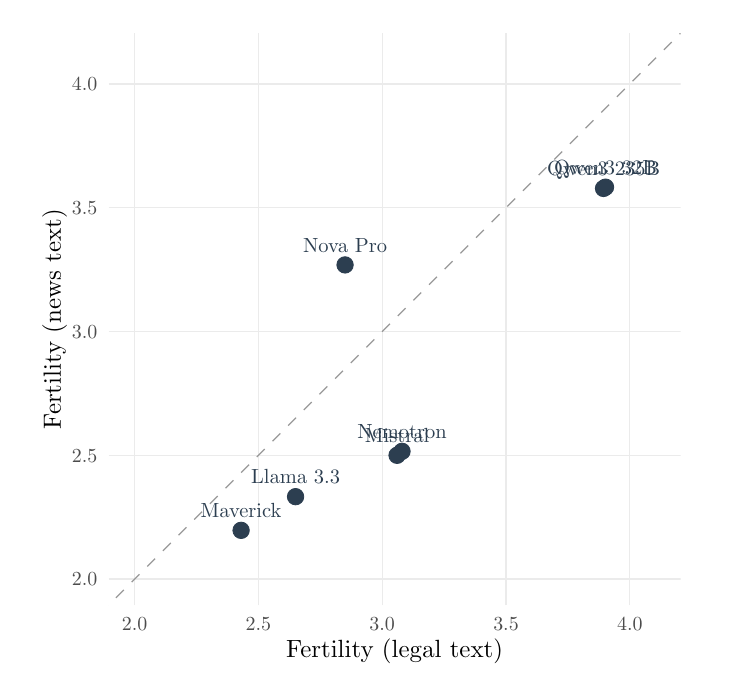
\begin{tikzpicture}[x=1pt,y=1pt]
\definecolor{fillColor}{RGB}{255,255,255}
\path[use as bounding box,fill=fillColor,fill opacity=0.00] (0,0) rectangle (245.72,231.26);
\begin{scope}
\path[clip] (  3.81,  0.00) rectangle (241.91,231.26);
\definecolor{fillColor}{RGB}{255,255,255}

\path[fill=fillColor] (  3.81,  0.00) rectangle (241.91,231.26);
\end{scope}
\begin{scope}
\path[clip] ( 29.25, 22.61) rectangle (235.91,229.26);
\definecolor{drawColor}{gray}{0.92}

\path[draw=drawColor,line width= 0.5pt,line join=round] ( 29.25, 32.00) --
	(235.91, 32.00);

\path[draw=drawColor,line width= 0.5pt,line join=round] ( 29.25, 76.73) --
	(235.91, 76.73);

\path[draw=drawColor,line width= 0.5pt,line join=round] ( 29.25,121.46) --
	(235.91,121.46);

\path[draw=drawColor,line width= 0.5pt,line join=round] ( 29.25,166.19) --
	(235.91,166.19);

\path[draw=drawColor,line width= 0.5pt,line join=round] ( 29.25,210.92) --
	(235.91,210.92);

\path[draw=drawColor,line width= 0.5pt,line join=round] ( 38.65, 22.61) --
	( 38.65,229.26);

\path[draw=drawColor,line width= 0.5pt,line join=round] ( 83.38, 22.61) --
	( 83.38,229.26);

\path[draw=drawColor,line width= 0.5pt,line join=round] (128.11, 22.61) --
	(128.11,229.26);

\path[draw=drawColor,line width= 0.5pt,line join=round] (172.84, 22.61) --
	(172.84,229.26);

\path[draw=drawColor,line width= 0.5pt,line join=round] (217.57, 22.61) --
	(217.57,229.26);
\definecolor{drawColor}{gray}{0.60}

\path[draw=drawColor,line width= 0.5pt,dash pattern=on 4pt off 4pt ,line join=round] (-177.40,-184.05) -- (442.57,435.92);
\definecolor{drawColor}{RGB}{44,62,80}
\definecolor{fillColor}{RGB}{44,62,80}

\path[draw=drawColor,line width= 0.3pt,line join=round,line cap=round,fill=fillColor] ( 77.12, 49.62) circle (  2.97);

\path[draw=drawColor,line width= 0.3pt,line join=round,line cap=round,fill=fillColor] (208.80,173.62) circle (  2.97);

\path[draw=drawColor,line width= 0.3pt,line join=round,line cap=round,fill=fillColor] ( 96.80, 61.79) circle (  2.97);

\path[draw=drawColor,line width= 0.3pt,line join=round,line cap=round,fill=fillColor] (133.48, 76.73) circle (  2.97);

\path[draw=drawColor,line width= 0.3pt,line join=round,line cap=round,fill=fillColor] (208.09,173.17) circle (  2.97);

\path[draw=drawColor,line width= 0.3pt,line join=round,line cap=round,fill=fillColor] (135.27, 78.16) circle (  2.97);

\path[draw=drawColor,line width= 0.3pt,line join=round,line cap=round,fill=fillColor] (114.69,145.53) circle (  2.97);

\node[text=drawColor,anchor=base,inner sep=0pt, outer sep=0pt, scale=  0.74] at ( 77.12, 54.23) {Maverick};

\node[text=drawColor,anchor=base,inner sep=0pt, outer sep=0pt, scale=  0.74] at (208.80,178.23) {Qwen3 32B};

\node[text=drawColor,anchor=base,inner sep=0pt, outer sep=0pt, scale=  0.74] at ( 96.80, 66.40) {Llama 3.3};

\node[text=drawColor,anchor=base,inner sep=0pt, outer sep=0pt, scale=  0.74] at (133.48, 81.34) {Mistral};

\node[text=drawColor,anchor=base,inner sep=0pt, outer sep=0pt, scale=  0.74] at (208.09,177.78) {Qwen3 235B};

\node[text=drawColor,anchor=base,inner sep=0pt, outer sep=0pt, scale=  0.74] at (135.27, 82.77) {Nemotron};

\node[text=drawColor,anchor=base,inner sep=0pt, outer sep=0pt, scale=  0.74] at (114.69,150.14) {Nova Pro};
\end{scope}
\begin{scope}
\path[clip] (  0.00,  0.00) rectangle (245.72,231.26);
\definecolor{drawColor}{gray}{0.30}

\node[text=drawColor,anchor=base east,inner sep=0pt, outer sep=0pt, scale=  0.72] at ( 25.20, 29.52) {2.0};

\node[text=drawColor,anchor=base east,inner sep=0pt, outer sep=0pt, scale=  0.72] at ( 25.20, 74.25) {2.5};

\node[text=drawColor,anchor=base east,inner sep=0pt, outer sep=0pt, scale=  0.72] at ( 25.20,118.98) {3.0};

\node[text=drawColor,anchor=base east,inner sep=0pt, outer sep=0pt, scale=  0.72] at ( 25.20,163.71) {3.5};

\node[text=drawColor,anchor=base east,inner sep=0pt, outer sep=0pt, scale=  0.72] at ( 25.20,208.44) {4.0};
\end{scope}
\begin{scope}
\path[clip] (  0.00,  0.00) rectangle (245.72,231.26);
\definecolor{drawColor}{gray}{0.30}

\node[text=drawColor,anchor=base,inner sep=0pt, outer sep=0pt, scale=  0.72] at ( 38.65, 13.60) {2.0};

\node[text=drawColor,anchor=base,inner sep=0pt, outer sep=0pt, scale=  0.72] at ( 83.38, 13.60) {2.5};

\node[text=drawColor,anchor=base,inner sep=0pt, outer sep=0pt, scale=  0.72] at (128.11, 13.60) {3.0};

\node[text=drawColor,anchor=base,inner sep=0pt, outer sep=0pt, scale=  0.72] at (172.84, 13.60) {3.5};

\node[text=drawColor,anchor=base,inner sep=0pt, outer sep=0pt, scale=  0.72] at (217.57, 13.60) {4.0};
\end{scope}
\begin{scope}
\path[clip] (  0.00,  0.00) rectangle (245.72,231.26);
\definecolor{drawColor}{RGB}{0,0,0}

\node[text=drawColor,anchor=base,inner sep=0pt, outer sep=0pt, scale=  0.90] at (132.58,  3.75) {Fertility (legal text)};
\end{scope}
\begin{scope}
\path[clip] (  0.00,  0.00) rectangle (245.72,231.26);
\definecolor{drawColor}{RGB}{0,0,0}

\node[text=drawColor,rotate= 90.00,anchor=base,inner sep=0pt, outer sep=0pt, scale=  0.90] at ( 12.01,125.94) {Fertility (news text)};
\end{scope}
\end{tikzpicture}
